\section{Integración y/o implementación de los componentes en la solución final}
\label{sec:integracion}

La carga vertical sigue la ruta rodamiento $\rightarrow$ revestimiento y apoyos sectoriales $\rightarrow$ viga central y travesaños de carga $\rightarrow$ uniones soldadas a momento $\rightarrow$ vigas longitudinales $\rightarrow$ ruedas $\rightarrow$ rieles $\rightarrow$ pedestales anclados $\rightarrow$ losa. Los centradores y los topes transmiten acciones laterales por caminos distintos; el pasador de bloqueo retiene la mesa en el sentido del recorrido en las dos estaciones, y la cadena la controla entre ellas. El distribuidor y su accionamiento cargan sobre el soporte superior, que es independiente de la cabina y de la mesa.

\subsection*{Secuencia de operación}

La operación separa el izaje, el centrado, el traslado y la aspersión, de modo que nunca coinciden dos movimientos peligrosos:
\begin{enumerate}
\item con el distribuidor detenido a $0^\circ$, la lanza retirada y la red sin presión, la mesa vacía se lleva con el volante a la estación de carga, fuera de la cabina, y se inserta el pasador en el receptor de carga;
\item el rodamiento se iza y se apoya sobre los tres apoyos sectoriales;
\item con la grúa sosteniendo parcialmente el aro, los centradores lo llevan contra las dos referencias y el empujador se detiene al alcanzar su fuerza normal; se activan los topes y se retira el aparejo;
\item se retira el pasador, la mesa se lleva con el volante a la estación de lavado, se inserta el pasador en el receptor de lavado y se retraen los centradores;
\item con la puerta cerrada y sin personal en la cabina, se baja la lanza y se ejecuta el lavado con el baño a 60--62~$^\circ$C;
\item la válvula de succión cambia al tanque de enjuague, se enjuaga y se deja escurrir;
\item se despresuriza la red, el distribuidor se detiene a $0^\circ$, se retira la lanza y la mesa vuelve a la estación de carga para retirar el rodamiento.
\end{enumerate}

El distribuidor solo puede girar, y la lanza bajar, con la mesa bloqueada en la estación de lavado. El traslado exige el distribuidor detenido a $0^\circ$, porque en las posiciones de $30^\circ$, $60^\circ$ y $90^\circ$ los barridos presentaron contacto. Estas condiciones se trasladan a los enclavamientos del Capítulo~\ref{cap:seguridad-ambiente}.

\subsection*{Interfaces}

La integración geométrica se verificó con barridos del modelo CAD en traslado, giro del distribuidor, retirada de la lanza y accionamiento de los centradores. La holgura vertical que gobierna en el modelo anterior es de 18,8 mm, entre el ala superior del bastidor ($Z=805$ mm) y los pies de la U ($Z=823{,}8$ mm), sin tolerancias aplicadas; en el modelo integrado final, el barrido del traslado completo no encontró choques (Sección~\ref{sec:representacion}). La Tabla~\ref{tab:interfaces-criticas} reúne las interfaces que condicionan la integración.

\begingroup
\footnotesize\singlespacing
\setlength{\parskip}{0pt}
\setlength{\tabcolsep}{4pt}
\renewcommand{\arraystretch}{1.05}
\begin{longtable}{@{}>{\raggedright\arraybackslash}p{2.8cm}>{\raggedright\arraybackslash}p{\dimexpr(\textwidth-2.8cm-2.2cm-6\tabcolsep)/2\relax}>{\raggedright\arraybackslash}p{\dimexpr(\textwidth-2.8cm-2.2cm-6\tabcolsep)/2\relax}>{\raggedright\arraybackslash}p{2.2cm}@{}}
\caption{Interfaces críticas de integración}\label{tab:interfaces-criticas}\\
\toprule
\textbf{Interfaz} & \textbf{Condición documentada} & \textbf{Verificación en la etapa de detalle} & \textbf{Estado}\\
\midrule\endfirsthead
\caption[]{Interfaces críticas de integración (continuación)}\\
\toprule
\textbf{Interfaz} & \textbf{Condición documentada} & \textbf{Verificación en la etapa de detalle} & \textbf{Estado}\\
\midrule\endhead
\midrule\multicolumn{4}{r}{\textit{Continúa en la página siguiente.}}\\\endfoot
\bottomrule\endlastfoot
Rodamiento--apoyos & Huella completa con error radial de 5 mm & Presión local, revestimiento y orientación del cono & Parcial\\
Mesa--distribuidor & Holgura de 18,8 mm; barrido del traslado sin choques & Holgura con tolerancias y flechas & Verificado en CAD nominal\\
Centradores--distribuidor & Sombra de los centradores retraídos sobre el diámetro exterior: visibilidad de 99,81 a 99,71\,\% & Efecto sobre la configuración de 24 boquillas & Parcial\\
Soporte--CFD & Los obstáculos del CAD coinciden con el modelo de mojado; las cartelas de los topes bajan la dosis como máximo un 0,19\,\% & Contrastar con la geometría final & Verificado\\
Rueda--riel & D/C 0,89 en servicio y 0,43 en estado último; fuerza lateral de 6,51 kN & Capacidad a baja velocidad y juego de la pestaña & Fabricante\\
Riel--losa & Pedestales con 4 anclajes M16; levantamiento de 3,78 kN & Losa real y producto adhesivo & Dato de planta\\
Distribuidor--soporte superior & Desplazamiento lateral del cojinete de 2,26 mm frente a 22,9 mm de holgura en el techo & Velocidad del motor frente a los modos del soporte & Verificado por simulación\\
Mesa--puerta & Recorrido de 3320 mm y paso por la puerta modelada & Levantamiento de planta y aparejo de grúa & Dato de planta\\
Bloqueo--control & Receptores de carga y lavado conectados al bastidor & Lógica de enclavamiento (Capítulo~\ref{cap:seguridad-ambiente}) & Definida en diseño\\
\end{longtable}
\endgroup

\subsection*{Circuito hidráulico}

El circuito se representó en un esquema de tuberías e instrumentación simplificado según ISO 10628-2, con 42 componentes e instrumentos (Figura~\ref{fig:esquema-hidraulico}). El agua del tanque de lavado pasa por la válvula de tres vías de succión, el colador y la bomba; sigue por la válvula de retención, la válvula de impulsión y el filtro de bolsa, sube por el montante hasta la unión rotativa y baja por el eje hueco hasta el cubo. Del cubo sale hacia la U, con 18 boquillas y sin válvulas de ramal, y hacia la lanza, con 6 boquillas, a través de una válvula de aislamiento y una manguera que sigue la carrera de 640 mm. El agua cae a la cabina y vuelve al tanque de lavado por el drenaje; para el enjuague, la válvula de succión cambia al tanque de 204 L. El esquema también representa el calentamiento del tanque, la dosificación del detergente y del inhibidor, el pozo de drenaje y un contenedor para la purga, como referencia de integración: esos elementos quedan fuera del alcance y no se dimensionaron. La hoja 2 del plano (Anexo~\ref{anx:planos}) señala para la etapa de detalle el tarado de la válvula de alivio, que comparte derivador con el caudal mínimo de la bomba, y la bolsa del filtro.

\begin{figure}[p]
\centering
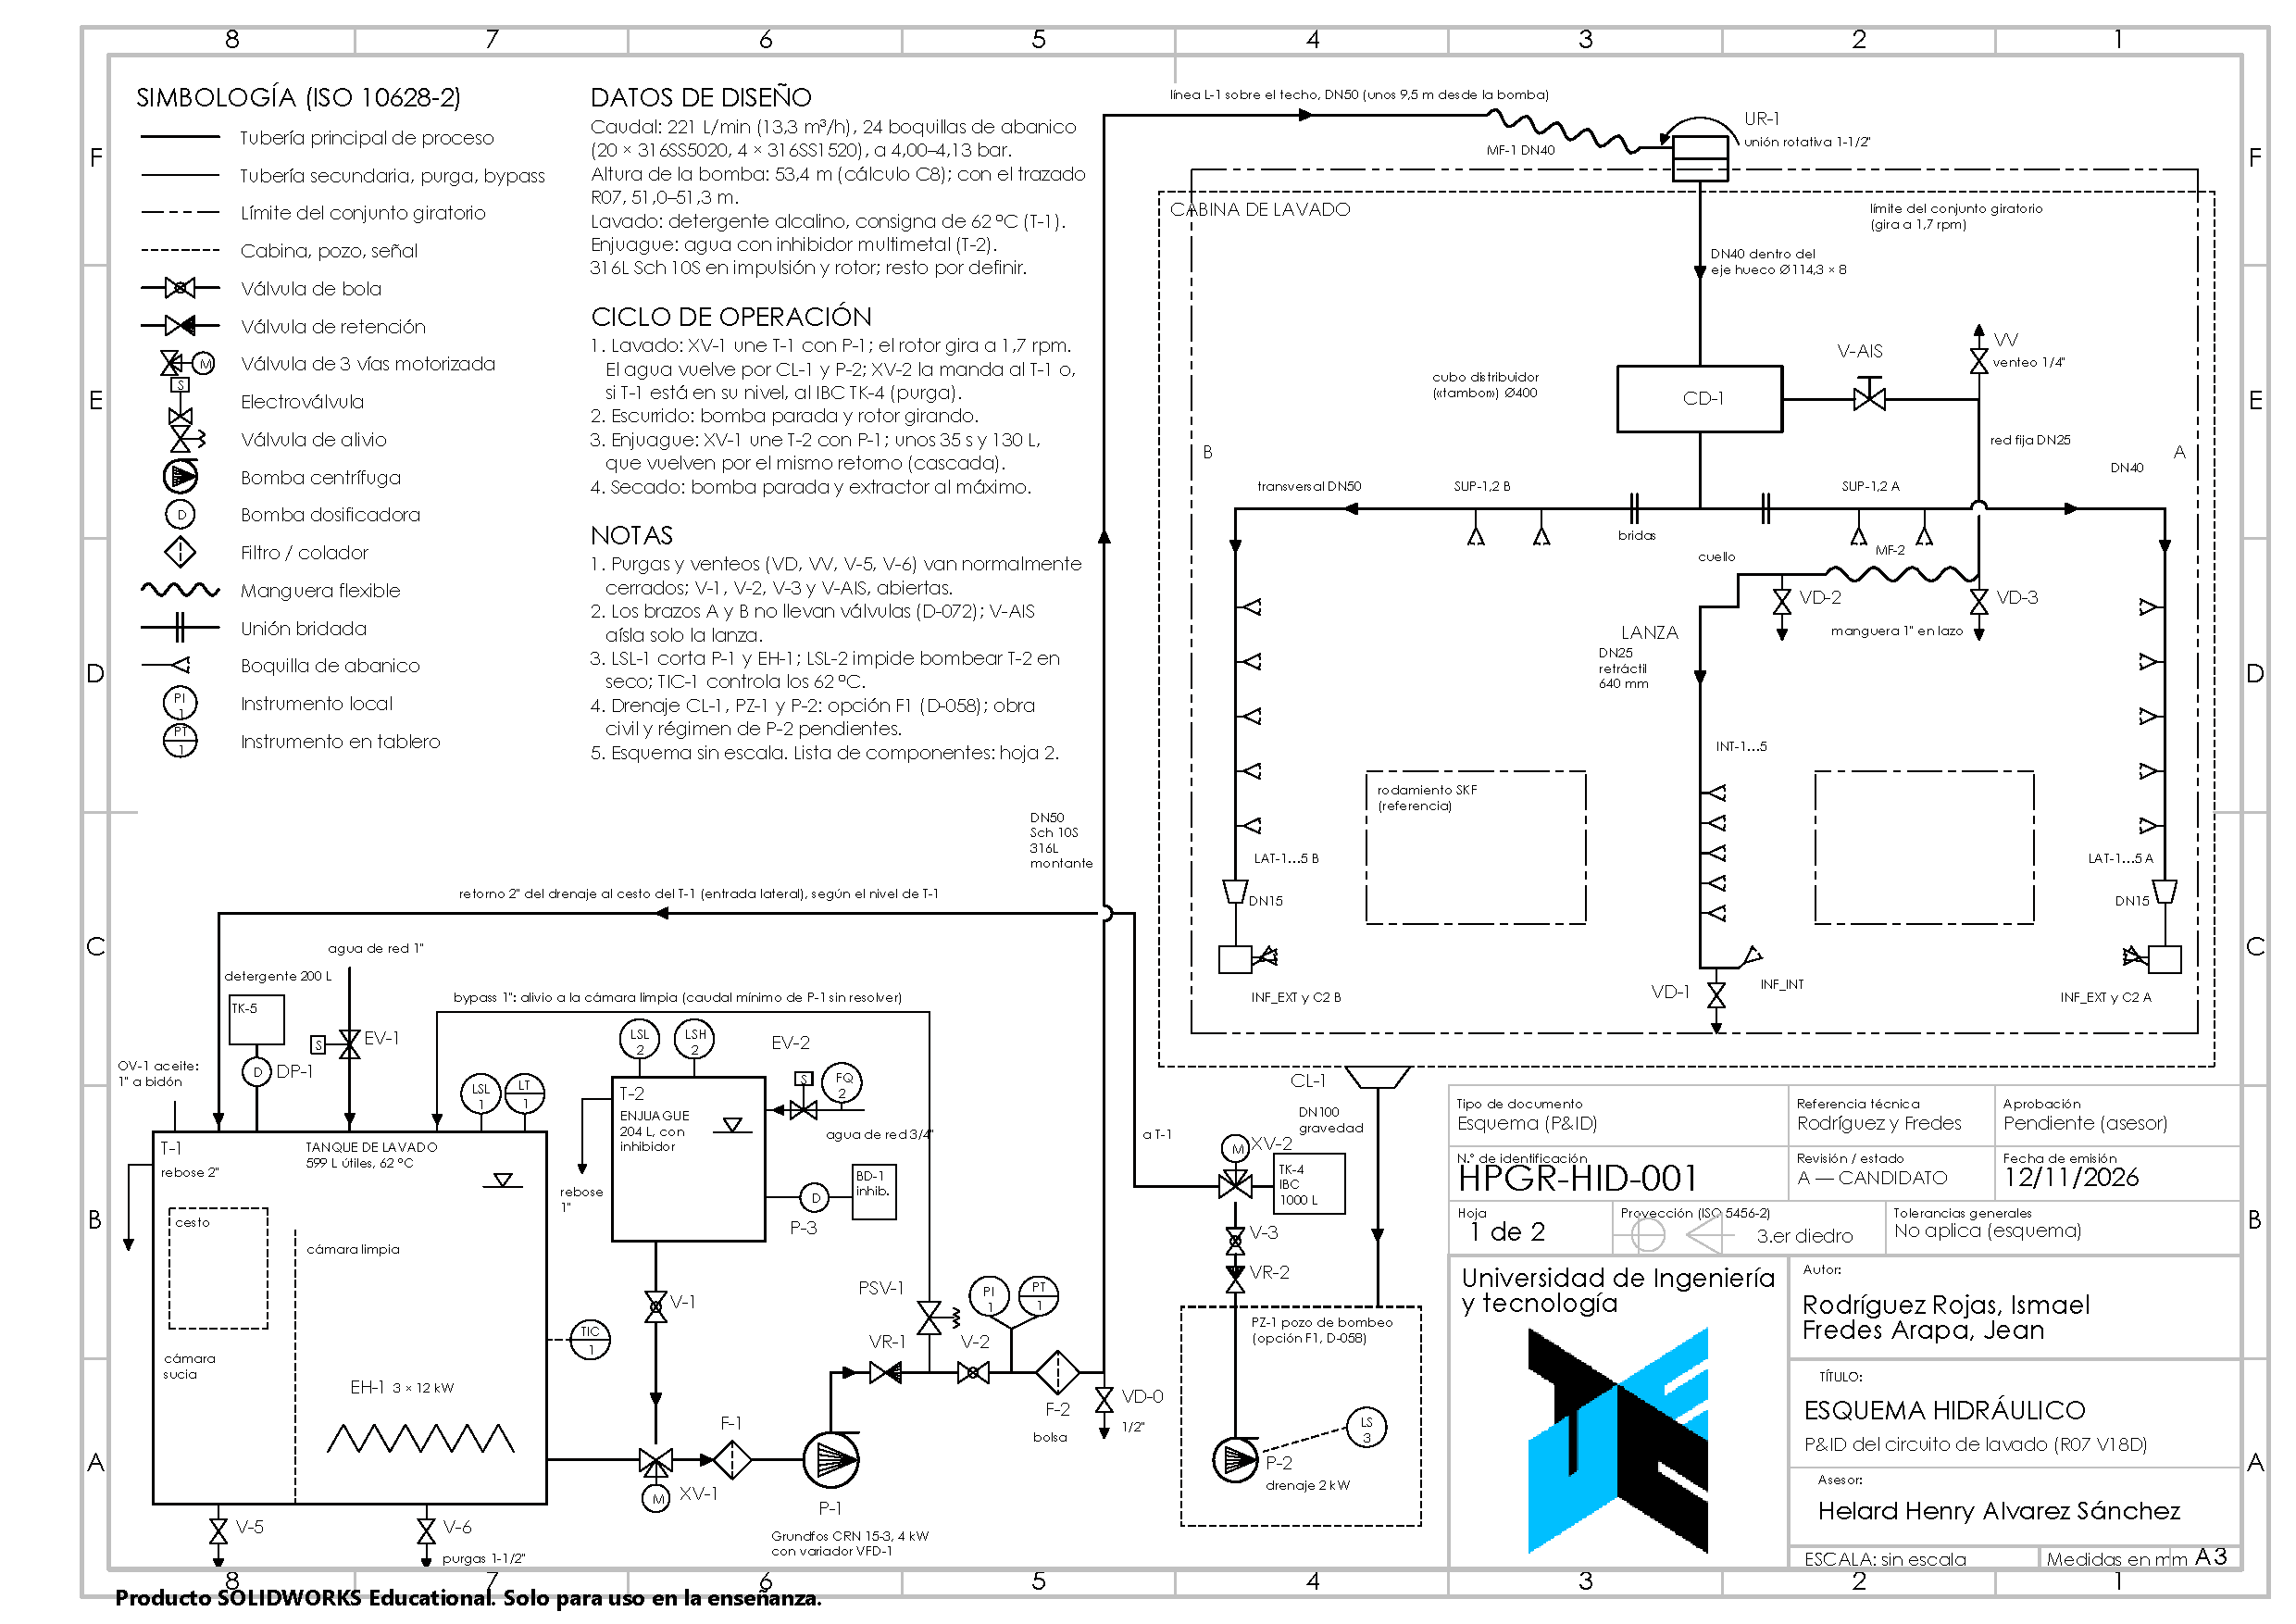
\includegraphics[angle=90,width=\textwidth,height=0.88\textheight,keepaspectratio]{HPGR-HID-001_hoja1.pdf}
\caption{Esquema hidráulico de la máquina, hoja 1: circuito, simbología, datos de diseño y ciclo. La hoja 2, con la lista de componentes, y el plano a tamaño completo están en el Anexo~\ref{anx:planos}. Elaboración propia en SolidWorks.}
\label{fig:esquema-hidraulico}
\end{figure}
